% !TEX root = ../main.tex

\chapter{三角贝赛尔曲面片表示的精确自由变形概述}
本文是在精确自由变形的基础上改进的一种方法,我们先来看一下精确自由变形的大概思路。

\section{定义变形空间}
精确自由变形选用的是B样条体作为变形空间,记作$\mathbf R(u,v,w)$。

\section{引言}
以下是一个测试用的列表环境,内容不要在意。\footnote{正文中中脚注命令测试,长脚注情况:这包括如下事实:“未经本人同意,监听、录制或转播私人性质的谈话或秘密谈话;未经本人同意,拍摄、录制或转播个人在私人场所的形象”}

这里测试列表标签功能的交叉引用格式\ref{itm:11},\ref{itm:12},\ref{itm:13},\ref{itm:14},分别表示第一至第四层级的itemize系列的交叉引用情况。
\begin{enumerate}
	\item 第一级列表\label{itm:11}
	\begin{enumerate}
		\item 第二级列表\label{itm:12}
	\end{enumerate}
\end{enumerate}

\begin{itemize}
	\item 第一级列表
	\begin{itemize}
		\item 第二级列表
	\end{itemize}
\end{itemize}

\section{浮动体测试}
\subsection{插图测试}
如\autoref{fig:first_image_tset}是对此模版的第一张插图测试。

\begin{figure}[htbp]
	\centering
	
\includegraphics[width = 0.5\linewidth]{Chapter1.png}
	\caption{第一张插图测试}\label{fig:first_image_tset}
\end{figure}

\subsection{表格测试}

\subsubsection{array宏包tabular表格环境测试}
如\autoref{tab:first_table_test}是对array宏包的tabular表格环境测试。
\begin{table}[htbp]
	\centering
	\caption{这是一个用tabular环境的测试用的表格}\label{tab:first_table_test}
    \begin{tabular}{lrr}
    \toprule
    \textbf{行星}     & \textbf{赤道半径}km & \textbf{公转周期}d \\
    \midrule
    水星     & 2.439  & 87.9 \\
    金星     & 6.1    & 224.682 \\
    地球     & 6378.14 & 365.24 \\
    \bottomrule
    \end{tabular}%
\end{table}

\subsubsection{tabu宏包表格环境测试}
如\autoref{tab:tabu_test_1}是对tabu宏包的tabu表格环境测试。在这里表格命令与\autoref{tab:first_table_test}的命令相同,只是tabular环境改成了tabu环境。
\begin{table}[htbp]
	\centering
	\caption{这是一个用tabu环境的测试用的表格}\label{tab:tabu_test_1}
    \begin{tabu}{lrr}
    \toprule
    \textbf{行星}     & \textbf{赤道半径}km & \textbf{公转周期}d \\
    \midrule
    水星     & 2.439  & 87.9 \\
    金星     & 6.1    & 224.682 \\
    地球     & 6378.14 & 365.24 \\
    \bottomrule
    \end{tabu}%
\end{table}

\autoref{tab:tabu_test_2}对tabu to表格的x列模式进行测试。在表格导言区中设置为X[1]X[2]X[2],表示这三列表格的列宽比值为1:2:2,总的表格宽度由tabu to环境设置,这里设置为0.6\textbackslash linewidth。相比于tabular环境,tabu环境的列宽设置方便许多。
\begin{table}[htbp]
	\centering
	\caption{tabu环境测试表格---X列模式}\label{tab:tabu_test_2}
    \begin{tabu} to 0.6\linewidth{X[1]X[2]X[2]}
    \toprule
    \textbf{行星}     & \textbf{赤道半径}km & \textbf{公转周期}d \\
    \midrule
    水星     & 2.439  & 87.9 \\
    金星     & 6.1    & 224.682 \\
    地球     & 6378.14 & 365.24 \\
    \bottomrule
    \end{tabu}%
\end{table}

特别需要注意的是,longtabu是基于longtable宏包开发的,所以在zjuthesis.cls文件中已经插入了longtable宏包。longtable环境的所有功能都可以在longtabu中使用,如\textbackslash endhead,\textbackslash endfirsthead,\textbackslash endfoot,\textbackslash endlastfoot,和\textbackslash caption等。具体用法请参见longtable和tabu宏包的相应文档。
\begin{longtabu}{lccc}
\caption{材料弹性模量及泊松比}\label{tab:tabu_test_3}\\
\toprule
名  称   & 弹性模量E/Gpa & 切变模量G/Gpa & 泊松比$\mu$ \\
\midrule%
\endfirsthead
\caption{材料弹性模量及泊松比(续)}\\
\toprule
名  称   & 弹性模量E/Gpa & 切变模量G/Gpa & 泊松比$\mu$ \\
\midrule%
\endhead
\bottomrule%
\endfoot
镍铬钢、合金钢 & 206    & 79.38  & 0.3 \\
碳 钢    &  196~206 & 79     & 0.3 \\
\end{longtabu}%

\subsection{子图}

如\autoref{fig:subfig_test1}是有两张子图的模式,对子图进行交叉引用,如\autoref{subfig:1a}和\autoref{subfig:1b}。

\begin{figure}[htbp]
	\centering
	\begin{subfigure}[b]{.4\textwidth}
		\centering
		
\includegraphics[width = \textwidth]{Chapter2.png}
		\caption{书籍排版与普通排版}\label{subfig:1a}
	\end{subfigure}
	\quad
	\begin{subfigure}[b]{.4\textwidth}
		\centering
		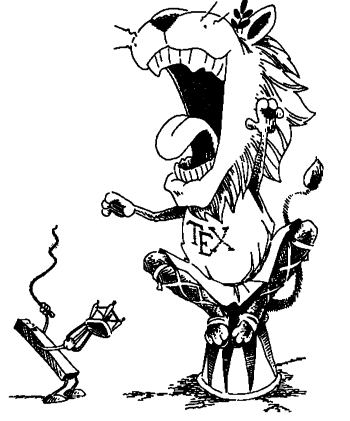
\includegraphics[width = \textwidth]{Chapter3.png}
		\caption{\TeX 的控制系列}\label{subfig:1b}
	\end{subfigure}
	\caption{子图模式测试1:2张图}\label{fig:subfig_test1}
\end{figure}

\begin{figure}[htbp]
	\centering
	\begin{subfigure}[b]{.4\textwidth}
		\centering
		
\includegraphics[width = \textwidth]{Chapter4.png}
		\caption{字体}\label{subfig:2a}
	\end{subfigure}
	\begin{subfigure}[b]{.4\textwidth}
		\centering
		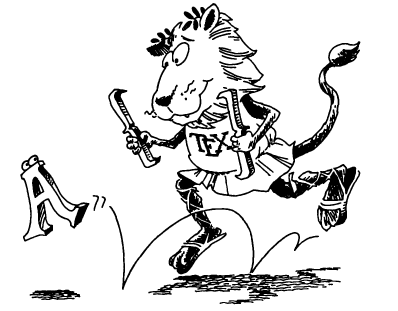
\includegraphics[width = \textwidth]{Chapter5.png}
		\caption{编组}\label{subfig:2b}
	\end{subfigure}
	\begin{subfigure}[b]{.4\textwidth}
		\centering
		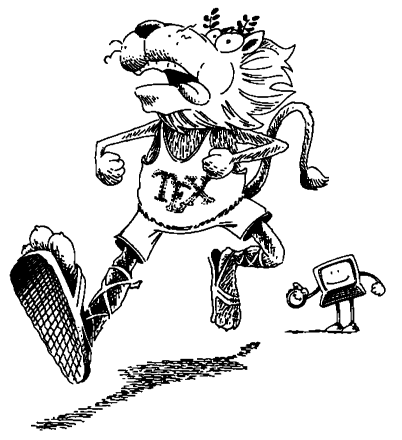
\includegraphics[width = \textwidth]{Chapter6.png}
		\caption{运行\TeX}\label{subfig:2c}
	\end{subfigure}
	\begin{subfigure}[b]{.4\textwidth}
		\centering
		
\includegraphics[width = \textwidth]{Chapter7.png}
		\caption{\TeX 工作原理}\label{subfig:2d}
	\end{subfigure}
	\caption{子图模式测试2:4张图}\label{fig:subfig_test2}
\end{figure}

\subsection{数学模式测试}
数学模式测试,主要测试数学字体,编号和交叉引用。这里首先推荐使用\texttt{align}和\texttt{align*}数学模式环境,大多数行间数学模式只需要用这个环境就可以了。

交叉引用测试,如交引用命令{\ttfamily \textbackslash eqref}和\texttt{\textbackslash ref}命令的区别。如公式\eqref{eq:test1},公式\ref{eq:test1}显示,\texttt{\textbackslash eqref}命令比\texttt{\textbackslash ref}命令的应用结果多了个括号。

如公式\eqref{eq:test3}是单行公式环境,查看公式\eqref{eq:test3}和\eqref{eq:test1}之间的区别,好像在单行公式中没什么区别。
\begin{align}\label{eq:test3}
	f(x) = 2(x + 1)^{2} - 1
\end{align}

\texttt{align}公式环境,用在单行中。
\begin{align}\label{eq:test1}
	f(x) = 2(x + 1)^{2} - 1
\end{align}

\begin{align*}
	f(x) = 2(x + 1)^{2} - 1
\end{align*}
在这里,中间插入一些文字以形成段落,查看行间公式与上下文之间的间隙。下一个公式\eqref{eq:test2}是一个公式组,它在“=”位置对齐。
\begin{align}\label{eq:test2}
	f(x) & = 2(x + 1)^{2} - 1\\
		 & = 2(x^{2} + 2x +1)-1\\
		 & = 2x^{2} + 4x + 1
\end{align}


\section{关于引用}
图表的引用通过{\ttfamily \textbackslash autoref} 命令即可,使用ST LaTeXTools 插件还能自动补全。如果要修改前缀,那么就用{\ttfamily \textbackslash recnewcommand \textbackslash figureautorefname\{好图\}}即可,详见hyperref宏包说明。
